\chapter{Noções preliminares}
\section{Convenções}
Vamos começar definindo algumas convenções de notação:
\begin{itemize}
    \item $|X|$ é a cardinalidade do conjunto $X$.
    \item $[n]=\{1,...,n\}$
    \item $A\setminus B = \{a\in A|a\notin B\}$
    \item Um $k$-conjunto é um conjunto de cardinalidade $k$ (e um $k$-subconjunto é um subconjuto de cardinalidade $k$)
    \item $\overline{pq}$ é o segmento de reta com extremos em $p$ e $q$.
    \item $\overrightarrow{pq}$ é o segmento de reta orientado com origem em $p$ e extremidade em $q$.
    \item $\overleftrightarrow{pq}$ é a reta que passa pelos pontos $p$ e $q$.
    \item $\Delta(a,b,c)=\{\alpha a+\beta b+\gamma c|\alpha+\beta+\gamma=1, \alpha>0, \beta>0, \gamma>0\}$ é o triângulo aberto com vértices $a$, $b$ e $c$ se $a$, $b$, $c$ não são colineares.
    \item $\Delta[a,b,c]=\{\alpha a+\beta b+\gamma c|\alpha+\beta+\gamma=1, \alpha\geq0, \beta\geq0, \gamma\geq0\}$ é o triângulo fechado com vértices $a$, $b$ e $c$ se $a$, $b$, $c$ não são colineares.
\end{itemize}

\section{Grafos}
Um grafo é um par $G=(V,E)$ em que $V$ é um conjunto enumerável (geralmente finito) e $E$ é um conjunto de pares não ordenados de elementos de $V$. Os elementos de $V$ são chamados \textbf{vértices}, e os elementos de $E$ são chamados \textbf{arestas}.

Se $G$ é um grafo, chamamos de $V(G)$ seu conjunto de vértices e de $E(G)$ seu conjunto de arestas.

Chamamos \textbf{ordem} de um grafo a cardinalidade de seu conjunto de vértices.

Se uma aresta $e=\{u,v\}\in E(G)$, dizemos que $u$ e $v$ são \textbf{vizinhos} ou \textbf{adjacentes}.

Um grafo \textbf{completo} é um grafo em que todos dois vértices distintos são adjacentes. Chamamos o grafo completo de ordem $n$ de $K_n$.

Se $G$ é um grafo e  $S\subset V(G)$ é um conjunto de vértices, chamamos de \textbf{subgrafo} de $G$ induzido por $S$ o grafo $G[S]=(S,E_S)$, em que $E_S=\{{u,v}\in E(G)|u,v\in S\}$. Nesse caso, dizemos que $G$ contém uma cópia de $G[S]$ ou simplesmente que $G$ contém $G[S]$, ou ainda que $G$ possui $G[S]$.

Uma \textbf{$k$-clique} é um conjunto de vértices $C$ tal que $G[C]$ é um grafo completo de ordem $k$.

Um grafo é \textbf{planar} se pode ser desenhado no plano sem que as curvas que representam as arestas se cruzem. Tal desenho é chamado de \textbf{imersão do grafo no plano}. Um grafo \textbf{plano} é um grafo planar com uma imersão no plano.

\section{Grafo de visibilidade}
Na sessão anterior, definimos conceitos básicos de teoria dos grafos. Aqui vamos estudar um caso bem particular.

Seja $P$ um conjunto de pontos no plano e $x,y\in P$. Dizemos que $x$ e $y$ são visíveis em $P$ se $\overline{xy}\cap P =\{x,y\}$. $p_1, p_2, ..., p_n$ são visíveis se são visíveis dois a dois.\footnote{Vamos considerar só conjuntos que são densos em nenhum lugar, i.e. o interior de $P$ é vazio.}

O grafo de visibilidade de um conjunto $P$ de pontos no plano é o grafo construído da seguinte forma: o conjunto de vértices é $P$ e há uma aresta entre dois vértices $x$ e $y$ se $x$ e $y$ são visíveis. Denotamos esse grafo por $\mathcal V(P)$ e se ${p,q}$ é uma aresta, às vezes nos referimos a ela como o segmento aberto $\overline{pq}$.

Dizemos que um grafo de visibilidade é plano se suas arestas não se interceptam.

\begin{teorema}[\cite{visibility}]\label{planork4}
    Todo grafo de visibilidade finito é plano ou contém uma cópia de $K_4$.
\end{teorema}
\begin{proof}
    Seja $G=\mathcal V(P)$ um grafo de visibilidade finito. Suponha que $G$ não seja plano. Vamos mostrar que $G$ contém $K_4$.

    Como $G$ não é plano, existe alguma aresta $\overline{ab}$ que intercepta com outras (pelo menos uma outra). A reta $\overleftrightarrow{ab}$ separa o plano em dois semiplanos $D$ e $E$. Seja $p$ o ponto de $D$ mais próximo do segmento $\overline{ab}$ e $q$ o ponto de $E$ mais próximo do segmento $\overline{ab}$ tal que $\overline{pq}$ intercepta $\overline{ab}$. Pela escolha de $p$ e $q$, os pontos $a$, $b$, $p$ e $q$ são visíveis, logo $G[\{a,b,p,q\}]$ é um $K_4$.
    \begin{center}
        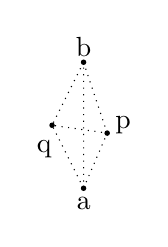
\begin{tikzpicture}
            \fill (0,0.2) circle (1pt);
            \fill (0,1.8) circle (1pt);
            \fill (0.3,0.9) circle (1pt);
            \fill (-0.4,1) circle (1pt);
            \draw[dotted] (0,0.2) -- (0,1.8) -- (0.3,0.9) -- (-0.4,1) -- (0,0.2);
            \draw [dotted] (0,0.2) -- (0.3,0.9);
            \draw [dotted] (0,1.8) -- (-0.4,1);
            \node (a) at (0,0) {a};
            \node (b) at (0,2) {b};
            \node (p) at (0.5,1) {p};
            \node (q) at (-0.5,0.7) {q};
        \end{tikzpicture}
    \end{center}
\end{proof}

\section {Teoria de Ramsey}

\subsection {Problema da festa}
Um bom problema para ilustrar a teoria de Ramsey é o problema da festa já mencionado:

\begin{problem}
    Qual a quantidade mínima de pessoas que deve haver em uma festa para que três delas se conheçam ou três delas não se conheçam?
\end{problem}

Vamos resolver esse problema usando teoria dos grafos.

Pessoas serão representadas por vértices e a relação entre elas por arestas coloridas. Se duas pessoas se conhecem, vamos colorir a aresta entre elas de azul, e se duas pessoas não se conhecem, vamos colorir a aresta entre elas de vermelho.

Reformulando a pergunta com essa formulação, temos:

\begin{problem}
    Qual o menor $n$ tal que toda coloração de arestas\footnote{Uma coloração de arestas de um grafo $G$ é uma função de $E(G)$ em um conjunto de cores, digamos $\{Azul, Vermelho\}$} de $K_n$ em $\{azul, vermelho\}$ possui uma 3-clique azul ou uma 3-clique vermelha (i.e. uma 3-clique com todas as arestas que ligam seus vértices azuis/vermelhas)?
\end{problem}

Vamos primeiro mostrar que $n=6$ resolve o problema e depois mostrar que $n=5$ não resolve, concluindo que $n=6$ é o mínimo.

\begin{prop}
    Toda coloração das arestas de $K_6$ possui uma 3-clique azul ou uma 3-clique vermelha.
\end{prop}
\begin{proof}
    Seja $x$ um vértice de $K_6$. Existem $5$ arestas com extremidade em $x$. Por contagem, pelo menos $3$ dessas arestas são da mesma cor, digamos, vermelhas. Sejam $a,b,c$ vértices tais que $xa,xb,xc$ são arestas coloridas de vermelho.

    Vamos olhar para as arestas $ab,bc,ca$. Se alguma delas for vermelha, temos um triângulo vermelho. Se nenhuma delas for vermelha, temos um triângulo azul. Isso prova que $n=6$ é sulficiente para resolver o problema.
\end{proof}

Para a seguinte coloração de $K_5$, não temos nenhuma 3-clique monocromática, logo $n=6$ é a solução desejada para o problema da festa.
\begin{center}
    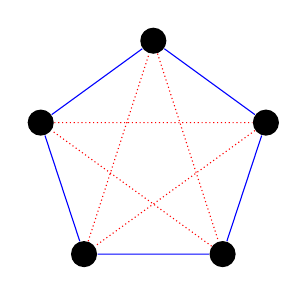
\begin{tikzpicture}
        \node[fill, circle] (V1) at (0,1.5) {};
        \node[fill, circle] (V2) at (1.43,0.46) {};
        \node[fill, circle] (V3) at (0.88,-1.21) {};
        \node[fill, circle] (V4) at (-0.88,-1.21) {};
        \node[fill, circle] (V5) at (-1.43,0.46) {};

        \draw[thin, color=blue] (V1) -- (V2) -- (V3) -- (V4) -- (V5) -- (V1);
        \draw[densely dotted, red] (V1) -- (V3) -- (V5) -- (V2) -- (V4) -- (V1);
    \end{tikzpicture}
\end{center}

\subsection {Teorema de Ramsey}
O teorema de Ramsey generaliza o resultado do problema da festa:

\begin{teorema}
    Para quaisquer $p,q\geq2$ inteiros existe um inteiro $N=R(p,q)$ tal que qualquer coloração de $K_N$ em duas cores possui uma $p$-clique azul ou uma $q$-clique vermelha.
\end{teorema}
\begin{proof}
    Vamos provar por indução em $p$ e $q$.

    Se $p=2$, uma coloração $K_N$ que não contém uma $2$-clique azul deve conter todas as arestas vermelhas. Mas então, para um $N\geq q$, essa coloração possui uma $q$-clique vermelha. Então $R(2,q)=q$. Da mesma forma, vemos que $R(p,2)=p$.

    Para mostrar que $R(p,q)$ existe para qualquer $p$ e $q$, vamos mostrar um limitante superior.

    Sejam $p,q\geq3$. Tome, como hipótese de indução, que $R(p,q-1)$ e $R(p,q-1)$ existam. Vamos mostrar que $R(p,q)\leq R(p,q-1)+R(p-1,q)$.

    Seja $N=R(p,q-1)+R(p-1,q)$ e $x$ um vértice de $K_N$. Considere os conjuntos dos vértices que são conectados a $x$ por uma aresta azul e dos que são conectados a $x$ por uma aresta vermelha. Chame-os de $A$ e $V$.

    Claramente $|A|+|V|=N-1=R(p,q-1)+R(p,q-1)-1$. Isso implica que ou $|A|\geq R(p,q-1)-1$ ou $|V|\geq R(p-1,q)-1$, pois caso contrário teríamos $|A|+|V|<R(p,q-1)+R(p-1,q)-2=N-2$.

    Suponha, sem perda de generalidade, que $|A|\geq R(p,q-1)-1$. Considere $K_{|A|}=K_N[A]$ o subgrafo induzido por $A$. Então um dos dois casos vale:
    \begin{itemize}
        \item $K_{|A|}$ contém uma $p$-clique vermelha.
        \item $K_{|A|}$ contém uma $(q-1)$-clique azul.
    \end{itemize}
    Se o primeiro caso for verdade, $K_N$ possui uma $p$-clique vermelha e não há nada a fazer.

    Se o segundo caso for verdade, como todas as arestas de $x$ a vértices de $A$ são azuis, considere os vértices da $(q-1)$-clique azul juntos com $x$. Esses vértices formam uma $q$-clique azul, então $K_N$ possui uma $q$-clique azul.
\end{proof}

\subsection {Generalizando para hipergrafos}
Assim como um grafo, um \textbf{hipergrafo $k$-uniforme} é um par $(V,E)$ em que $V$ é o conjunto de \textbf{vértices} e $E$ é o conjunto de \textbf{arestas}, só que os elementos de $E$ são $k$-subconjuntos de $V$.

O teorema de Ramsey pode ser generalizado da seguinte forma:

\begin{teorema}
    Para quaisquer $k>0$, $p,q\geq k$ inteiros, existe um inteiro $N=R^k(p,q)$ tal que para qualquer coloração das $k$-arestas do hipergrafo $k$-uniforme completo de $N$ vértices existe um conjunto de $p$ vérices tal que todas as $k$-arestas entre eles são azuis ou um conjunto de $q$ vértices tal que todas as $k$-arestas entre eles são vermelhas (alternativamente, para qualquer coloração dos $k$-subconjuntos de $\{1,...,N\}$ existe um $p$-subconjunto cujos $k$-subconjuntos são azuis ou um $q$-subconjunto cujos $k$-subconjuntos são vermelhos).
\end{teorema}
\begin{proof}
    Vamos mostrar por indução em $p$, $q$ e $k$.

    Primeiramente, se $k=1$, é fácil ver que $R^k(p,q)=max\{p,q\}$, já que as colorações são de vértices individuais.

    Agora, se $p=k$, uma coloração que não contém um conjunto de $p=k$ vértices com as arestas azuis tem que conter todas as arestas vermelhas. Similarmente à base da indução no caso de grafos, temos que $R^k(k,q)=q$ e, por simetria, $R^k(p,k)=p$.

    Sejam $p,q,k$ como no enunciado do teorema. Pela hipótese de indução, para qualquer $x,y$ existem:
    \begin{itemize}
        \item $R^{k-1}(x,y)$
        \item $R^k(p-1,y)$
        \item $R^k(x,q-1)$
    \end{itemize}
    Vamos mostrar que existe $R^k(p,q)$.

    Seja $N=R^{k-1}(R^k(p-1,q),R^k(p,q-1))+1$. Considere $K^N_k$ o hipergrafo $k$-uniforme completo de $N$ vértices e uma coloração $\chi$ de suas arestas.

    Escolha um vértice qualquer $x$ e seja $S$ a coleção de todas as $(k-1)$-arestas que não contêm $x$. $S$ define um hipergrafo $(k-1)$-uniforme completo de $N-1$ vértices e possui uma coloração induzida por $\chi$ dada por $\chi'(e)=\chi(e\cup\{x\})$ para toda aresta $e$ de $S$. 
    
    Pela escolha de $N$, podemos aplicar nossa hipótese de indução em $S$ e colcluir que vale:
    \begin{itemize}
        \item Ou $S$ tem um conjunto $A$ de $R^k(p,q-1)$ vértices tal que toda (k-1) aresta de $S$ em $A$ é azul (para $\chi'$);
        \item Ou $S$ tem um conjunto $V$ de $R^k(p-1,q)$ vértices tal que toda (k-1) aresta de $S$ em $V$ é vermelha (para $\chi'$).
    \end{itemize}
    Sem perda de generalidade, suponha que o primeiro caso que vale.

    Então, pela hipótese de indução, vale uma das seguintes afirmações:
    \begin{itemize}
        \item A tem um $(p-1)$-subconjunto $T$ tal que toda $k$-aresta em $T$ é azul (para $\chi$)
        \item A tem um $q$-subconjunto $T$ tal que toda $k$-aresta em $T$ é vermelha (para $\chi$)
    \end{itemize}
\end{proof}

No segundo caso o teorema está provado. Olhando para o primeiro caso, considere $T'=T\cup\{x\}$. Se uma aresta $a$ em $T'$ contém $x$, ela é azul por que $a\setminus x$ foi pintado de azul em $S$ por $\chi'$. Se uma aresta e $T'$ não contém $x$, então ela também está em $T$ e, por hipótese, é azul. Assim $T'$ é um conjunto de $p$ vértices com todas as arestas nele azuis.

\section{Geometria combinatória}
Vamos dar algumas definições a respeito de conjuntos de pontos no plano. Seja $P$ um conjunto finito de pontos no plano e $conv(P)$ o casco convexo de $P$. Dizemos que $P$ está em \textbf{posição geral} se não existirem três pontos colineares em $P$. 

Dizemos que $P$ está em \textbf{posição convexa} se todo ponto de $P$ estiver na fronteira de $conv(P)$.

Um ponto $v\in P$ é um \textbf{vértice} de $P$ se $conv(P)\neq conv(P\backslash v)$.

Se todos os pontos de $P$ forem vértices, dizemos que $P$ está em \textbf{posição estritamente convexa}.

Um \textbf{$k$-ágono} é o casco convexo de um conjunto de $k$ pontos em posição estritamente convexa.

Se $X$ for um subconjunto de $P$ de $k$ pontos em posição estritamente convexa tal que $conv(X)\cap P=X$, então  $conv(X)$ é um \textbf{$k$-buraco} ou um \textbf{$k$-ágono vazio}.

Uma \textbf{triangulação} de um $k$-ágono $T$ é um conjunto de $3$-ágonos tal que os vértices dos $3$-ágonos também são vértices de $T$, $T$ é a união de todos os $3$-ágonos e a interseção de quaisquer dois $3$-ágonos tem área $0$.

Chamamos $3$-ágonos de triângulos, $4$-ágonos de quadriláteros, $5$-ágonos de pentágonos, etc.

\subsection{Teorema de Erd\H os-Szekeres}
Um resultado clássico da teoria de Ramsey na geometria combinatória é o seguinte:
\begin{teorema}[Erd\H os-Szekeres, 1935]
    Dado um inteiro positivo $k$, existe um inteiro $ES(k)$ tal que todo conjunto com pelo menos $ES(k)$ pontos em posição geral contém $k$ pontos em posição estritamente convexa.
\end{teorema}

Vamos mostrar uma demonstração dada por \cite{ES} e, para isso, primeiro vamos resolver um caso particular com $k=5$:
\begin{lema}
    Todo conjunto com $5$ pontos em posição geral contém quatro pontos em posição estritamente convexa.
\end{lema}
\begin{proof}
    Seja $P$ um conjunto com $5$ pontos em posição geral. Se $conv(P)$ for um pentágono ou um quadrado, o lema é trivial.
    Então vamos supor que $conv(P)$ seja um triângulo. Tal triângulo possui dois pontos de $P$, $u$ e $v$, em seu interior. A reta que contém esses dois pontos separa os vértices do triângulo, dois ($p$ e $q$) de um lado e um ($x$) do outro lado. Então $\{u,v,p,q\}$ são quatro pontos em posição estritamente convexa.
\end{proof}

Agora podemos demonstrar o teorema:
\begin{proof}(Teorema de Erd\H os-Szekeres)
    Dado um $k$ inteiro positivo, considere $P$ um conjunto com pelo menos $R^4(k,5)$ pontos em posição geral. Para cada subconjunto $X$ de $P$ de tamanho $4$, vamos colorí-lo de vermelho se $conv(X)$ for um quadrilátero e de azul de $conv(X)$ for um triângulo. Pelo teorema de Ramsey para hipergrafos, uma das duas condições é satisfeita:
    \begin{itemize}
        \item $P$ tem um subconjunto de tamanho $k$ tal que todo subconjunto dele com 4 elementos é vermelho.
        \item $P$ tem um subconjunto de tamanho $5$ tal que todo subconjunto dele com 4 elementos é azul.
    \end{itemize}
    Pelo lema, a segunda opção não é possível, pois ela implicaria que um conjunto com $5$ pontos não tem 4 pontos em posição estritamente convexa. Então existe um subconjunto de tamanho $k$ tal que todo subconjunto dele com $4$ elementos é vermelho. Seja $H$ tal conjunto.

    Vamos mostrar que $H$ está em posição estritamente convexa. Para isso, suponha o contrário. Então existe algum ponto $x$ de $H$ no interior de $conv(H)$. Considere uma triangulação de $conv(H)$. $x$ está dentro de algum triângulo da triangulação. Os três vértices desse triângulo juntos com $x$ formam um conjunto de $4$ pontos que deveria ter sido pintado de azul, o que é uma contradição.

    Logo $H$ é um conjunto de $k$ pontos em posição estritamente convexa.
\end{proof}

\subsection{Teorema de Sylvester-Gallai}
Outro resultado interessante é o teorema de Sylvester-Gallai. A seguinte demonstração é de \cite{Kelly1986}.


\begin{teorema}
    Todo conjunto finito de pontos tem todos os pontos colineares ou existe uma reta que passa por exatamente dois desses pontos.
\end{teorema}
\begin{proof}
    Seja $P$ um conjunto finito de pontos no plano tal que $P$ não tem todos os pontos colineares e seja $\mathcal L$ o conjunto ds retas com pelo menos dois pontos de $P$.

    Como $P$ é finito, existe $p\in P$ e $L\in\mathcal L$ tais que a distância de $p$ a $L$ é mínima.

    Vamos mostrar que $|P\cap L|\leq 2$.
    \begin{center}
        \begin{tikzpicture}
            \filldraw (0,2) circle[radius=1.5pt];
            \node at (0.1,2.5) (p) {$p$};
            \draw[dashed] (-4,0) -- (4,0);
            \node at (-1,-0.5) (L) {$L$};
            \filldraw (1,0) circle[radius=1.5pt];
            \node at (1,0.5) (x) {$x$};
            \filldraw (3,0) circle[radius=1.5pt];
            \node at (3.1,0.5) (y) {$y$};
            \draw[dashed] (4.5,-1) -- (-1.5,3);
            \node at (1.5,1.5) (L') {$\overleftrightarrow{py}$};
        \end{tikzpicture}
    \end{center}

    Suponha o contrário, que $P$ contém pelo menos 3 pontos em $L$.

    A reta perpendicular a $L$ que passa por $p$ separa $L$ em duas semirretas. Uma dessas semirretas tem que conter pelo menos $2$ pontos de $P$, pois caso contrário $|P\cap L|\leq 2$. Vamos nomear esses pontos de $x$ e $y$, com $x$ mais próximo de $p$ do que $y$.

    Mas então a distância $x$ a $\overleftrightarrow{py}$  é menor que a distância de $p$ a $L$, contrdizendo a escolha de $p$ e $L$.
\end{proof}

